\section{Bancos de dados relacionais}

Bancos de dados relacionais são sistemas que implementam o modelo de dados
relacional proposto por Codd na década de 70 \cite{Codd1970}, rapidamente
implementado por um sistema chamado System R da IBM \cite{Astrahan1976}.
A principal ideia é a de representar os dados em forma de relações (tabelas)
e as operações são definidas a partir de uma álgebra: a álgebra relacional.
O sistema recebe comandos através de uma linguagem declarativa (SQL) 
\cite{Chamberlin1974}, os converte em operadores da álgebra relacional
para então poder ser executada nos dados persistentes nas relações.

\begin{figure}
        \centering
        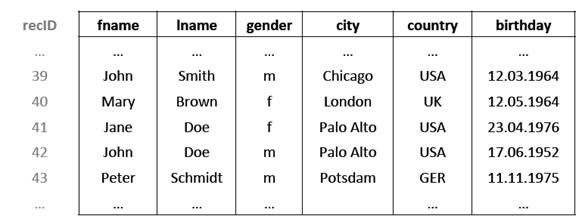
\includegraphics[width=\linewidth]{./colunar_repr_tabela.png}
        \caption{Representação de uma tabela em um banco de dados relacional.}
        \label{fig:tabular}
\end{figure}

A Figura \ref{fig:tabular} mostra a representação de uma relação contendo 
informações sobre indivíduos em um formato de tabela. Esta relação possui
os seguintes atributos do indivíduo : (i) \emph{fname}, o nome; (ii) 
\emph{lname}, o sobrenome; (iii) \emph{gender}, o sexo, \emph{m} para 
masculino e \emph{f} para feminino; (iv) \emph{city},
a cidade onde nasceu; (v) \emph{country}, o país onde nasceu; e 
(vi) \emph{birthday}, a data de nascimento.

Os principais operadores da álgebra relacional são: projeção ($\Pi$),
seleção ($\sigma$), junção ($\bowtie$). Sejam duas relações $R$ e $S$
com atributos $r_1, \ldots, r_m$ e $s_1, \ldots, s_n$, representadas
por $R(r_1, \ldots, r_m)$ e $S(s_1, \ldots, s_n)$. Uma projeção em $R$
recebe como argumento uma lista de atributos subconjunto dos atributos
de $R$ e retorna a relação contendo somente os atributos desta lista.
A projeção é representada por $\Pi_{lista~de~atributos}(R)$. Uma seleção
em $R$ recebe como argumentos uma condição em forma de predicado e 
retorna todas as tuplas em $R$ que satisfazem o predicado. A seleção 
é representada por $\sigma_{predicado} (R)$. A junção é um operador
binário e é aplicado sobre duas relações $R$ e $S$, recebe como argumento
uma condição em forma de predicado (usualmente a igualdade entre dois
atributos das relações $R$ e $S$), e retorna a relação correspondente
ao produto cartesiano das duas relações $R$ e $S$ cujas tuplas satisfazem
o predicado da junção. A junção é representada por $R \bowtie_{predicado} S$. 

A linguagem SQL expressa de forma declarativa operações sobre os dados
armazenados nas relações a partir da álgebra relacional. Uma versão simplificada
da linguagem SQL é mostrada a seguir:

\begin{lstlisting}[style=MySQLStyle]
SELECT <lista de atributos>
FROM   <lista de tabelas>
WHERE  <predicado>;
\end{lstlisting}

Após o sistema receber uma consulta na linguagem SQL, esta deve ser expressada
segundo operadores da álgebra relacional da forma mais eficiente possível. Um 
otimizador de consultas é o responsável por esta tradução. A ordem dos operadores
influencia no resultado; normalmente seleções ($\sigma$) são as primeiras a serem
executadas, pois reduzem o tamanho das relações resultantes. A ordem das junções
também é de extrema importância; uma junção entre as relações $R$, $S$ e $T$ pode
ser executada nas seguintes ordens: (i) $R \bowtie S \bowtie T$, (ii) 
$R \bowtie T \bowtie S$ e (iii) $S \bowtie T \bowtie R$. Adicionalmente, existem
inúmeros algoritmos para a execução eficiente das junções que devem coexistir no
sistema e serem utilizados em circunstâncias em que são os mais eficientes 
\cite{Mishra1992}.

O problema da contagem de triângulos da Seção \ref{triangles} pode ser expresso na 
seguinte consulta SQL, assumindo que temos uma relação chamada Twitter com os attributos
\emph{follower} e \emph{followee} contendo números inteiros de identificadores de usuários
representando relacionamentos na rede social, onde \emph{follower} segue \emph{followee}.

\begin{lstlisting}[style=MySQLStyle]
SELECT COUNT(*) 
FROM   TWITTER R, TWITTER, S, TWITTER T
WHERE  R.followee = S.follower AND
       S.followee = T.follower AND
       T.followee = R.follower AND
       R.follower > S.follower AND
       S.follower > T.follower;
\end{lstlisting}

Uma forma de execução desta consulta, em operadores da álgebra relacional é 
\begin{multline}
\sigma_{S.follower > T.follower}(\sigma_{R.follower > S.follower}(( R \bowtie_{R.followee = S.follower} S ) \\
\bowtie_{(S.followee = T.follower) \land (T.followee = R.follower)} T))
\end{multline}

Este plano de execução irá seguir os seguintes passos:

\begin{enumerate}
\item Primeira junção entre as tabelas $R$ e $S$ com predicado $R.followee = S.follower$
\item Seleção com predicado $R.follower > S.follower$ aplicado ao resultado anterior
\item Junção do resultado anterior com a tabela $T$ com predicado $(S.followee = T.follower) \land (T.followee = R.follower)$
\item Seleção com predicado $S.follower > T.follower$
\end{enumerate}
